\chapter{Agile}
\section{Agile}
\subsection{Metodologia Agile}
Costruire sistemi safety-critical, governativi o gestire molti team distribuiti sul territorio richiede una
coordinazione efficace. Verso la fine degli anni '90, il contesto di sviluppo software è cambiato radicalmente.
I piani rigidi non erano più sempre efficaci, specialmente considerando le richieste di consegne sempre più rapide.
Con team piccoli, l'overhead generato da processi pesanti sarebbe stato un costo eccessivo, portando così all'adozione
di una metodologia Agile.

Il requisito fondamentale nella metodologia Agile è rispondere rapidamente ai cambiamenti anziché seguire pedissequamente
un piano preciso. Data l'incertezza sulle esigenze finali e la loro probabile evoluzione nel corso dello sviluppo,
l'Agile propone una strategia per gestire tali cambiamenti. In questo contesto, si evita di congelare i requisiti
iniziali, ma si cerca piuttosto di capire meglio cosa si vuole ottenere.

Nella metodologia Agile, la specifica, il design e l'implementazione procedono in parallelo e sono strettamente collegati.
Il software finale viene gestito attraverso una serie di versioni, con ciascuna versione successiva che rappresenta un
incremento del prodotto. È cruciale coinvolgere il cliente e gli stakeholder durante tutto il processo di sviluppo Agile
in modo da assicurare un feedback costante e un allineamento continuo con le aspettative,
dotandosi di strumenti informali di comunicazione.

Di solito, si stabilisce un intervallo di tempo limitato per lo sviluppo di ciascuna versione, che va da 2 a 4 settimane.
La documentazione è mantenuta al minimo per evitare discrepanze e inconsistenze tra la documentazione e il codice stesso.
La comunicazione all'interno del team è spesso informale ma frequente, promuovendo un flusso costante di informazioni.

Per automatizzare il processo di testing, è fondamentale adottare strumenti per il testing automatico, in quanto il testing
manuale risulterebbe troppo lento e inefficiente data la necessità di coprire numerosi scenari di test. Alcuni strumenti
chiave per la metodologia Agile includono:

\begin{itemize}
    \item Testing automatico
    \item Gestione della configurazione
    \item Integrazione continua
    \item Produzione automatica dell'interfaccia utente
\end{itemize}

L'obiettivo è rilevare e correggere gli errori il prima possibile, in modo da evitare che si propaghino attraverso il sistema.

\subsection{Manifesto Agile}
L'Agile si basa su alcuni principi chiave che sono riassunti nel Manifesto Agile:

\begin{itemize}
    \item L'importanza è spostata dal processo formale all'individuo e alle interazioni
    che i membri devono avere.
    \item È più importante avere un software funzionante rispetto a una documentazione esaustiva.
    \item Si promuove la collaborazione con il cliente, che dovrebbe essere parte integrante
    del team di sviluppo piuttosto che
    un soggetto esterno con cui contrattare.
    \item L'attenzione è posta sulla capacità di rispondere al cambiamento in modo rapido e flessibile, piuttosto che
    sull'aderenza rigorosa a un piano prestabilito.
\end{itemize}

\subsection{Implementazione della metodologia Agile}
\subsubsection{Coinvolgimento del Cliente}
Per realizzare appieno i principi dell'Agile, è fondamentale coinvolgere attivamente il cliente nel processo di sviluppo.
Il coinvolgimento del cliente deve andare oltre il semplice fornitore di specifiche, incoraggiando il cliente a partecipare
attivamente alle discussioni e al processo decisionale. Questo assicura che le funzionalità sviluppate siano allineate con
le aspettative del cliente e che i feedback siano integrati tempestivamente nel processo di sviluppo.
\subsubsection{Sviluppo Incrementale}
Un altro aspetto chiave è lo sviluppo incrementale, dove le funzionalità vengono fornite in maniera graduale e integrata
nel sistema in crescita. 
\subsubsection{Persone e non Processi}
In questo contesto, è fondamentale avere team con competenze solide e diversificate, che si fidino
a vicenda per garantire un flusso di lavoro efficiente e un'efficace condivisione delle
responsabilità.
\subsubsection{Risposta al Cambiamento}
Nella metodologia Agile, è importante prepararsi al cambiamento continuo dei requisiti nel corso del progetto. La capacità di
adattarsi rapidamente ai nuovi requisiti e di integrarli nel processo di sviluppo è un fattore cruciale per il successo.
\subsubsection{Semplicità}
Il principio cardine per lo sviluppo Agile è quello di mantenere la semplicità. Ciò implica resistere alla tentazione di
aggiungere funzionalità non essenziali che potrebbero introdurre una complessità eccessiva nel sistema. L'obiettivo è quello
di adottare strategie che semplifichino il processo e riducano al minimo il rischio di complicazioni impreviste durante lo
sviluppo.

\subsection{Applicabilità della metodologia Agile}
La metodologia Agile è particolarmente adatto in contesti in cui il cliente è disponibile e desideroso di partecipare attivamente
al processo di sviluppo del software. È efficace in ambienti in cui le normative sono meno restrittive e permettono una maggiore
flessibilità nel processo di sviluppo. I processi di sviluppo Agile sono spesso implementati in combinazione con metodologie di
gestione progetti agili, come ad esempio Scrum.

\section{Extreme Programming (\texttt{XP})}
Spesso, nell'ambito della metodologia Agile, si fa riferimento a \textbf{Extreme Programming}, che spinge all'estremo
alcune delle caratteristiche fondamentali dell'Agile. Ad esempio, in Extreme Programming, sono comuni varie versioni del software
consegnate al cliente quotidianamente, con incrementi che vengono immediatamente messi in produzione. Un principio chiave è che i
casi di test devono superare con successo per ogni build, pertanto è necessario assicurarsi che tutti i casi di test siano funzionanti
prima di procedere con una nuova build.

Nel contesto di Extreme Programming, viene dato ampio risalto alla pratica di scrivere i test prima di scrivere il codice effettivo.
Il refactoring è una pratica costante con l'obiettivo di semplificare il codice sorgente per renderlo più leggibile e mantenibile nel
tempo. Altro aspetto fondamentale di \texttt{XP} include il pair programming, in cui due sviluppatori lavorano insieme su un singolo codice,
garantendo una maggiore qualità e condivisione delle conoscenze. Inoltre, si mira a mantenere un ritmo di sviluppo sostenibile nel tempo,
evitando eccessive accelerazioni che potrebbero compromettere la qualità del software.

\section{User Stories}
Nel contesto dell'Agile, i requisiti vengono spesso raccolti in maniera informale tramite user stories, che sono narrazioni in prosa
che descrivono le interazioni tra l'utente e il sistema. Questo metodo aiuta a mantenere i requisiti concreti e facilita l'elicitazione
dei requisiti stessi poiché le user stories sono facili da scrivere e da comprendere.

Le user stories vengono successivamente suddivise in parti più piccole, comunemente chiamate task cards. Per ogni task, è necessario
fornire una stima temporale per la sua realizzazione. L'obiettivo è quello di coinvolgere attivamente il cliente nella priorizzazione
delle varie attività, poiché, in un contesto di sviluppo incrementale, non è possibile affrontare tutto contemporaneamente.

Tuttavia, con questo tipo di approccio, non si ha la certezza di implementare tutte le funzionalità richieste, poiché alcune di esse
potrebbero non emergere in determinati scenari o iterazioni di sviluppo.
\subsubsection{Esempio di User Story}
\begin{tcolorbox}[title ={Prescrizione}]
    Kate è un medico che desidera prescrivere farmaci per un paziente che sta
    frequentando una clinica. Il record del paziente è già visualizzato sul suo
    computer, quindi fa clic sul campo dei farmaci e può selezionare \textit{farmaci attuali},
    \textit{nuovi farmaci} o \textit{formulario}.
    Se seleziona \textit{farmaci attuali}, il sistema le chiede di controllare la dose;
    Se vuole modificare la dose, inserisce la nuova dose e quindi conferma la prescrizione.
    Se sceglie \textit{nuovi farmaci}, il sistema presume che lei sappia quale farmaco
    prescrivere. Digita le prime lettere del nome del farmaco. Il sistema visualizza un
    elenco di possibili farmaci che iniziano con queste lettere. Lei sceglie il farmaco
    richiesto e il sistema risponde chiedendole di verificare che il farmaco selezionato
    sia corretto. Inserisce la dose e quindi conferma la prescrizione.
    Se sceglie \textit{formulario}, il sistema visualizza una casella di ricerca per
    il formulario approvato. Può quindi cercare il farmaco richiesto. Seleziona un farmaco
    e le viene chiesto di verificare che il farmaco sia corretto. Inserisce la dose e
    quindi conferma la prescrizione.

    Il sistema controlla sempre che la dose sia nell'intervallo approvato. Se non lo è,
    a Kate viene chiesto di cambiare la dose.
    Dopo che Kate ha confermato la prescrizione, questa verrà visualizzata per il controllo.
    Lei fa clic su \textit{OK} o \textit{Modifica}. Se fa clic su \textit{OK},
    la prescrizione viene registrata nel database di audit. Se fa clic su \textit{Modifica},
    riprende il processo di \textit{Prescrizione di farmaci}.
    
\end{tcolorbox}

\subsubsection{Esempio di Task Card}
\begin{tcolorbox}[title ={Task 1: Controllo della dose}]
Il controllo della dose è una precauzione di sicurezza per verificare che il medico
non abbia prescritto una dose pericolosamente piccola o grande.
Utilizzando l'identificativo del formulario per il nome del farmaco generico,
consultare il formulario e recuperare la dose massima e minima raccomandata.
Controllare la dose prescritta rispetto al minimo e al massimo. Se è al di fuori
dell'intervallo, emettere un messaggio di errore che indica che la dose è troppo
alta o troppo bassa. Se è all'interno dell'intervallo, abilitare il pulsante ``Conferma''.
\end{tcolorbox}

\section{Test-Driven Development (\texttt{TDD})}
Nel Test-Driven Development (\texttt{TDD}), i test vengono scritti prima del codice stesso, e tali test possono essere eseguiti durante la fase
di scrittura del codice. Questo approccio consente di individuare errori il prima possibile, valutando ogni singola microcomponente
prima di passare a quella successiva. Il codice risultante è di alta qualità in quanto viene costantemente testato e non presenta bug
evidenti.

I test, in questo contesto, rappresentano una documentazione degli scenari previsti e consentono di pensare al comportamento del sistema
prima ancora di implementarlo effettivamente. Ciò porta a una maggiore consapevolezza del sistema e del suo funzionamento da parte del
team di sviluppo.

Inoltre, è importante coinvolgere attivamente l'utente nella fase di verifica, in modo da sviluppare i cosiddetti acceptance test per le
varie user stories. Questo è possibile solo grazie all'utilizzo di framework di test automatizzati. Di conseguenza, il numero di test
generati è notevolmente elevato, garantendo la coerenza e la stabilità del sistema, specialmente in un contesto di sviluppo incrementale.

\subsection{Refactoring}
Il refactoring rappresenta il processo di riscrittura del codice al fine di renderlo più leggibile e mantenibile nel lungo periodo.
Spesso, ogni singolo incremento potrebbe richiedere alcuni compromessi che, per essere integrati nel sistema, richiedono una sorta di
``degradazione" del sistema. Il refactoring permette di affrontare tali problematiche e di mantenere l'integrità del sistema nel tempo,
assicurandone la stabilità e la longevità. Il refactoring risulta essere una pratica altrettanto valida anche nel contesto di sviluppo
pianificato (\textit{plan-driven}).

\subsection{Pair Programming}
Il pair programming è una pratica in cui due persone lavorano insieme su un singolo computer. Mentre una persona scrive il codice,
l'altra controlla attivamente il lavoro. I ruoli si alternano regolarmente, e le decisioni cruciali vengono prese in modo collaborativo.
I vantaggi del pair programming sono numerosi, inclusa la condivisione della responsabilità, il controllo continuo e un feedback costante.
Inoltre, il continuo scambio di conoscenze e la code review continua portano a un miglioramento delle abilità individuali e della qualità
del codice. Il refactoring continuo contribuisce ulteriormente a migliorare la comunicazione all'interno del team. Contrariamente a ciò
che si potrebbe pensare, il pair programming non causa una diminuzione significativa della produttività, ma piuttosto conduce a un miglioramento
generale delle prestazioni del team.
\section{\texttt{CI/CD} nel Sviluppo Software Moderno}

\texttt{CI/CD} è un acronimo che sta per ``Continuous Integration'' (\textit{Integrazione Continua})
e ``Continuous Delivery'' o ``Continuous Deployment'' (\textit{Consegna Continua o Distribuzione Continua}). Questi sono concetti chiave nelle pratiche di
sviluppo software moderno, in particolare nell'ambito della metodologia Agile e DevOps.

\subsection{Continuous Integration (\texttt{CI})}
La Continuous Integration si riferisce alla pratica di integrare automaticamente i cambiamenti del codice nel repository principale di un progetto
più volte al giorno. Il suo scopo è identificare e risolvere rapidamente i problemi di compatibilità o altri problemi introdotti da nuove modifiche.
Questo processo coinvolge tipicamente l'uso di strumenti automatizzati per compilare e testare il codice ogni volta che un cambiamento viene \textit{committato},
assicurando che il codice nuovo funzioni correttamente con il codice esistente.

\subsection{Continuous Delivery (\texttt{CD})}
La Continuous Delivery si estende dalla \texttt{CI} e implica la consegna automatica di cambiamenti del codice a un ambiente di test o di produzione dopo il
processo di integrazione. L'obiettivo è rendere il processo di rilascio del software il più efficiente e prevedibile possibile, riducendo i tempi
e i costi di distribuzione.

\subsection{Continuous Deployment}
Il Continuous Deployment è simile al Continuous Delivery. Tuttavia, mentre nel Continuous Delivery ogni rilascio richiede ancora un'intervento
manuale per la distribuzione in produzione, nel Continuous Deployment ogni cambiamento che passa tutte le fasi di produzione viene rilasciato
automaticamente senza intervento umano.

\section{Project Management Agile}
Nel contesto della metodologia Agile, il project manager ha la responsabilità di assicurarsi che il software venga consegnato entro i tempi
previsti, con tutte le funzionalità richieste e nel rispetto del budget stabilito. È responsabile del coordinamento del progetto e del
monitoraggio dei progressi.

\subsection{Scrum}
Scrum è un metodo di project management agile che si basa sul lavoro per iterazioni, richiamando così il processo di sviluppo software agile.
Le sue fasi principali includono:

\begin{enumerate}
    \item Definizione di obiettivi generali e architettura ad alto livello del sistema.
    \item Sprint planning, in cui si definiscono gli obiettivi per la prossima iterazione.
    \item Fase conclusiva, dove si ``incarta'' il progetto,
    si completa la documentazione finale, si esegue code review e
    si riflette sulle lezioni apprese.
\end{enumerate}

\subsubsection{Terminologia}
Di seguito sono riportati alcuni termini chiave in Scrum:

\begin{center}
\begin{tabular}{|p{4cm}|p{9cm}|}
\hline
\textbf{Termine} & \textbf{Descrizione} \\
\hline
Team piccolo & Gruppo di massimo $7$ persone, ottimale per favorire la comunicazione diretta e l'agilità nelle attività. \\
\hline
Incremento & Ogni incremento corrisponde a un prodotto consegnabile al cliente, completo e testato. Ad esempio, se ci sono link, devono essere cliccabili e funzionanti. \\
\hline
Product Backlog & Lista di tutte le funzionalità che il prodotto deve avere, utilizzata come ``to-do list" per il team di sviluppo. \\
\hline
Product Owner & Cliente, committente o stakeholder che fa parte del team e ha il compito di priorizzare le funzionalità, rappresentando le esigenze degli utenti finali. \\
\hline
Scrum & Meeting giornaliero veloce, noto anche come stand-up meeting, per verificare il progresso del team e priorizzare le attività. \\
\hline
Sprint & Periodo di lavoro di $2$-$4$ settimane, durante il quale il team si impegna a consegnare un incremento di funzionalità. \\
\hline
Scrum Master & Responsabile del monitoraggio e del supporto al processo di sviluppo, garantisce che il team segua le regole di Scrum. \\
\hline
Velocità & Produttività del team, misurata durante lo sviluppo, che indica quanti elementi del backlog il team è in grado di sviluppare durante uno sprint. \\
\hline
Sprint Review & Sessione in cui il team riflette sull'iterazione appena conclusa e fornisce input per migliorare i prossimi sprint. \\
\hline
\end{tabular}
\end{center}

\subsubsection{Ciclo di sviluppo Scrum}
\begin{figure}[H]
    \centering
    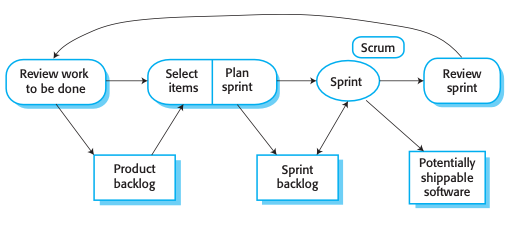
\includegraphics[scale=0.6]{img/sprintcycle.png}
    \caption{Ciclo di sviluppo Scrum}
\end{figure}
Si parte con la definizione del Product Backlog, che è una lista di tutte le
funzionalità che il prodotto deve avere. Il product owner è responsabile di
priorizzare le funzionalità, in modo da inserire in cima alla lista quelle più
importanti per il cliente.

Per farlo tipicamente si utilizzano task board, in cui
si possono visualizzare le attività da svolgere, le attività relative allo 
sprint non ancora iniziate, le attività in corso e le attività in rilascio. 

Le attività con più alta priorità verranno inserite nello sprint backlog, che è
la lista di attività che il team si impegna a completare entro la fine dello
sprint. Il numero di attività inserite nello sprint backlog è determinato dalla
velocità del team, ovvero dalla produttività del team, stimata inizialmente e 
calibrata durante lo sviluppo.

Durante lo sprint, il team si impegna a completare le attività dello sprint
backlog, e si tiene un meeting giornaliero veloce, noto anche come scrum,
per verificare il progresso del team e priorizzare le attività. Di norma 
la durata di uno sprint è di $2$-$4$ settimane e questa durata viene stabilita all'inizio 
del progetto e non viene modificata.

Durante queste due settimane il team lavora in modo autonomo, senza comunicare 
con il cliente. Tutte le comunicazioni con il product owner avvengono
tramite lo scrum master, che ha il compito di mediare la comunicazione tra
il team e il cliente.

Durante lo scrum meeting, l'obiettivo è comunicare ciò che verrà fatto 
nella giornata corrente, riassumendo ciò che è stato fatto il giorno precedente
e identificando eventuali ostacoli che impediscono il completamento delle attività.

Al termine dello sprint, il team si riunisce per riflettere sull'iterazione appena
conclusa e fornire input per migliorare i prossimi sprint. Questa sessione è
nota come sprint review. Se alcune attività non vengono completate
entro la fine dello sprint, vengono inserite nel backlog e verranno riproposte
nello sprint successivo.

\subsubsection{Benefici}
I benefici di Scrum includono la gestione efficiente di funzionalità nel breve termine,
una conoscenza approfondita
dei problemi e delle attività di ogni membro del team, nonché la puntualità delle consegne
per il cliente. Scrum favorisce
un clima di fiducia tra il cliente e il team di sviluppo, poiché il cliente ha la possibilità
di visualizzare il sistema software
funzionante e fornire un feedback continuo. Questo feedback aiuta a chiarire le esigenze
del cliente e ad adattare il prodotto
in modo efficace.

\subsection{Scrum Distribuito}
Lo Scrum distribuito si riferisce a situazioni in cui il team di sviluppo è distribuito
in più sedi geografiche.
È importante che il product owner faccia visita agli sviluppatori in modo da stabilire 
una relazione di fiducia e a garantire che il team sia allineato con le esigenze del cliente.
In questo contesto, la comunicazione tra i membri del team avviene attraverso strumenti
come chat in tempo reale, chiamate video.
La continuous integration server per garantire che il software sia sempre funzionante 
e pronto per il rilascio, in modo che i membri del team siano in grado si sincronizzare
e lavorare in modo collaborativo.
È importante adottare un ambiente di sviluppo condiviso, in modo che tutti i membri del team
possano accedere alle stesse risorse e strumenti di sviluppo.
\section{Scalabilità delle metodologie Agili}
Abbiamo detto che tipicamente le metodologie agili sono adatte a progetti di piccole
dimensioni, dove gli sviluppatori sono collocati nella stessa sede e i progetti sono 
di piccola e media dimensione. Tuttavia, è possibile adattare le metodologie agili
a progetti di grandi dimensioni, dove gli sviluppatori sono distribuiti in più sedi
geografiche lavorando anche in più team di sviluppo, e i progetti durano per più tempo.

Quando viene applicata la scalabilità è importante mantenere i fondamenti agili relativi a:
\begin{itemize}
    \item Pianificazione flessibile
    \item Rilasci frequenti
    \item Continuous integration
    \item Test driven development
    \item Buona comunicazione tra i membri del team
\end{itemize}
È inoltre importante coordinare lo sviluppo agile con esigenze del post-sviluppo, ovvero 
della manutenzione del software. Per le caratteristiche viste, la metodologia di sviluppo 
agile prevede una documentazione minima, ma quando viene affrontata la manutenzione del
software, è necessario avere una documentazione più dettagliata, perché il team di manutenzione
potrebbe non essere lo stesso team di sviluppo. Le problematiche principali che si incontrano
sono che i sistemi sviluppati con metodologie agili potrebbero essere \textbf{difficili da
mantenere},
perché la documentazione può essere non allineata con il codice, e quando i membri 
del team originale lasciano l'azienda, la conoscenza del sistema potrebbe andare persa.
\subsection{Problematiche nell'adozione delle metodologie agili}
In generale potrebbero verificarsi delle problematiche legate all'adozione di metodologie
agili.
\subsubsection{Problematiche di sistema}
Quando si adotta una metodologia agile è importante chiedersi:
\begin{itemize}
    \item Quanto grande sarà il sistema? I metodi agili sono adatti a
    sistemi dove gli sviluppatori sono collocati nella stessa sede,
    in modo da comunicare in maniera non formale e i progetti
    sono di piccola e media dimensione.
    \item Che tipologia di sistema si sta sviluppando? I metodi agili
    sono adatti a sistemi dove non è richiesta una grossa analisi 
    iniziale prima di iniziare lo sviluppo.
    \item Quanto sarà la vita del sistema? Solitamente i progetti 
    di lunga durata richiedono una documentazione più dettagliata
    rispetto a quelli di breve durata, e i metodi agili prevedono
    una documentazione minima.
    \item Il sistema è soggetto a regolamentazioni? I metodi agili
    sono adatti a sistemi dove non è richiesta una grossa documentazione
    per soddisfare regolamentazioni.
\end{itemize}
\subsubsection{Problematiche legate al team}
\begin{itemize}
    \item Il supporto tecnologico è adeguato? I metodi agili richiedono
    un ambiente di sviluppo condiviso, in modo che tutti i membri del team
    possano accedere alle stesse risorse e strumenti di sviluppo. È necessario 
    che gli \texttt{IDE} supportino la visualizzazione e l'analisi del codice
    se la documentazione è minima. 
    \item Il team è competente? È necessario
    che il team sia formato e competente in modo da poter prendere decisioni
    in maniera autonoma.
    \item Come è organizzato il team? Se le persone sono tutte insieme 
    allora possono decidere in maniera coordinata le decisioni da prendere.
    In caso di team distribuiti, è necessario adottare una documentazione 
    più dettagliata.
\end{itemize}
\subsubsection{Problematiche legate all'organizzazione}
\begin{itemize}
    \item Come è organizzato il lavoro? Se il lavoro è organizzato in modo
    gerarchico, potrebbe essere difficile adottare metodologie agili. 
    \item Come è la cultura aziendale? Inoltre,
    la comunicazione informale può o meno far parte del profilo aziendale.
    \item Il cliente è coinvolto? È necessario che il cliente sia disponibile 
    per fornire un feedback continuo, senza feedback continuo il team di sviluppo
    non riuscirà a capire le esigenze del cliente e adottare un cambiamento 
    dei requisiti in modo efficace.
\end{itemize}
\subsection{Metodi agili per sistemi di grandi dimensioni}
Nel contesto dello sviluppo di sistemi software complessi, è comune
incontrare la necessità di adattare le metodologie agili per gestire sfide specifiche.
Questo può verificarsi, ad esempio, quando si lavora su un ``sistema di sistemi", ovvero
un insieme di sistemi software che interagiscono tra loro e possono essere sviluppati da
più team.

Le situazioni che richiedono questa personalizzazione includono:

\begin{enumerate}
    \item \textbf{Configurazione anziché sviluppo orientato al codice:} In alcuni contesti,
    come quelli in cui la configurazione è più rilevante rispetto allo sviluppo del codice,
    è necessario adattare le pratiche agili per gestire efficacemente questo processo.
    
    \item \textbf{Regolamentazioni e documentazione dettagliata:} In presenza di molte
    regolamentazioni, è fondamentale avere una documentazione dettagliata. Le metodologie
    agili possono essere adattate per integrare questo requisito, assicurando che la
    documentazione sia adeguatamente gestita e aggiornata durante il processo di sviluppo.
    
    \item \textbf{Lunghezza dei contratti e rischio di perdere figure chiave:} In situazioni
    in cui i contratti sono estesi e vi è il rischio che figure chiave lascino il progetto
    prima del suo completamento, è necessario adottare approcci che garantiscano una gestione
    efficace delle risorse umane e una transizione fluida tra i membri del team.
    
    \item \textbf{Diversi stakeholder e rappresentanza:} Quando ci sono diversi stakeholder
    con interessi e requisiti vari, è importante disporre di rappresentanti per ogni categoria
    di stakeholder. Le metodologie agili possono essere personalizzate per includere meccanismi
    di coinvolgimento degli stakeholder e per gestire efficacemente le loro diverse esigenze e
    aspettative.
\end{enumerate}
\subsubsection{Scaling up}

Nel caso di software di grandi dimensioni, che richiedono l'impiego di più team di
sviluppo, è essenziale adottare un approccio strategico per gestire i requisiti e
l'implementazione del sistema. Un approccio incrementale potrebbe non essere
praticabile in questo contesto, pertanto è consigliabile una trattazione iniziale
dei requisiti seguita dall'implementazione.

Date le dimensioni del sistema, non è realistico assegnare la responsabilità di
product owner a una singola persona. È essenziale coinvolgere rappresentanti di
tutte le tipologie di stakeholder per garantire che i requisiti siano adeguatamente
compresi e considerati durante lo sviluppo.

Inoltre, in sistemi di grandi dimensioni, non è sufficiente fare affidamento
esclusivamente sul codice sorgente. È necessario documentare e stabilizzare
l'architettura e le parti critiche del sistema in modo da consentire lo sviluppo
indipendente dei vari componenti.

La comunicazione tra i team di sviluppo è fondamentale per garantire un allineamento
coerente e coeso del sistema. Questo assicura che il lavoro di ogni team sia complementare
e che il sistema complessivo sia sviluppato in modo armonico.

L'implementazione della continuous integration potrebbe risultare complessa in un sistema
di grandi dimensioni, poiché richiederebbe una verifica continua di ogni singola linea di
codice per garantire il corretto funzionamento complessivo del sistema. Tuttavia, è
possibile pianificare momenti specifici per integrare e testare i vari componenti del
sistema per garantire la coerenza e l'integrità complessiva del sistema.

\subsection{Multi-team Scrum}
In un contesto di multi-team Scrum, ciascun team è strutturato con un
Product Owner, responsabile della massimizzazione del valore del prodotto,
e uno ScrumMaster, responsabile di facilitare il processo
Scrum e rimuovere eventuali ostacoli che ostacolano il progresso del team.

Per garantire una coerenza nell'architettura del sistema, ogni team dispone
di un architetto del prodotto. Gli architetti del prodotto lavorano in collaborazione,
discutendo e definendo l'architettura complessiva del sistema. Questa collaborazione
assicura che il sistema sia progettato
in modo coerente e che soddisfi i requisiti di tutti gli stakeholder coinvolti.

Per massimizzare il valore del prodotto e garantire una migliore gestione dei
rischi, le date di rilascio del prodotto per tutti i team sono allineate.
Questo permette di produrre un sistema dimostrabile e completo, evitando
dispersione di risorse e assicurando che il prodotto soddisfi le aspettative
degli utenti e degli stakeholder.

Per mantenere un'efficace comunicazione e coordinazione tra i team, viene
organizzato un ``Scrum of Scrums" giornaliero. In questo incontro, i
rappresentanti di ciascun team si riuniscono per discutere i progressi,
le sfide e pianificare il lavoro da svolgere. Questo permette di identificare
tempestivamente eventuali problemi e risolverli in
modo collaborativo, garantendo il successo del progetto nel suo complesso.